\documentclass{article}
\usepackage{color}
\usepackage{xspace}
\usepackage{listings}
\usepackage{curves}
\usepackage{url}

\usepackage[pdftex]{graphicx}  

\title{Getting Started with Overlog and P2}
\author{Joe Hellerstein \and Petros Maniatis}

\begin{document}
\date{}
\maketitle

%% Overlog definition adapted from 
%% Prolog definition (c) 1997 Dominique de Waleffe
%%
\lstdefinelanguage{Overlog}%
  {morekeywords={materialize,periodic,insert,delete,keys},%
   sensitive=f,%
   morecomment=[s]{/*}{*/},%
   morestring=[bd]",%
   morestring=[bd]'%
  }[keywords,comments,strings]%

\lstset{language=Overlog,
        basicstyle=\small\sffamily,
%        stringstyle=\ttfamily,
        keywordstyle=\color{blue}\bfseries,
%        numbers=left, numberstyle=\tiny, stepnumber=1, numbersep=5pt
}

	
This document is an informal introduction to programming the P2
overlay network engine via its declarative language, Overlog.  After
reading this document and working through the examples, you should
be ready to try writing Overlog programs of your own.

\section{The Basics: Relations and Tuples}
Overlog is a logic programming language designed for specifying
distributed protocols and algorithms as overlay networks.  As with
other logic languages, the most basic concept in Overlog is the {\em
  relation}, which is like a database table: a set of
(unordered) but similarly-structured rows called {\em tuples}.  A
relation is described by a list of fields, and a tuple in the
relation is an assignment of values to each of the fields.  Data types
for the fields are simple scalars like integers, floats, and so
on. Fields with ``structured'' types -- such as
nested tuples or relations -- are not explicitly available in the
language, though they can be emulated if necessary.

Overlog differs from relational databases in having two types of
relations: traditional ``materialized'' (stored) relations, and
{\em streaming} relations.  Tuples in a streaming relation can be thought of
as events -- they are handled by Overlog logic as they are generated,
but once handled they are discarded.  Tuples in a materialized
relation are stored for subsequent use; materialized relations can be
configured either for long-term storage, or as ``soft state,'' with a
lifetime for each tuple before it expires and is deleted.

Another distinction between Overlog and relational tables is that
Overlog requires each tuple to have a network address embedded in it.
This is done by designating a field in a tuple as the \emph{location
  specifier}; location specifiers are typically strings of the form
``IP:port'' though others, such as multicast addresses or content-based
names are also possible; a tuple is intended to appear at the
address specified in its location specifier. 

As an example, an Overlog program might define a network link relation
named \lstinline$link$ with two string-valued fields: one for the
source IP:port pair, and another for the destination IP:port pair.  An
example tuple from this relation would be notated in Overlog as
follows:
\begin{lstlisting}
link("127.0.0.1:10000", "127.0.0.1:10001").
\end{lstlisting}

Within an Overlog program, a tuple of the \lstinline$link$ relation
might have its first or its second fields designated as the location
specifier. In the former case, a \lstinline$link$ tuple is intended to
appear at its source node, whereas in the latter it is intended to
appear at its destination node.



\section{Overlog Rules: The Ping-Pong Example}
\label{sec:pingPong}
Given that introduction on the basics of the Overlog data model, it's
time to write our first Overlog program.  This program will simply get
two machines to ``ping'' each other periodically, and acknowledge the
pings with ``pong'' messages.

Overlog programs are constructed from {\em rules}, which specify how
tuples are generated from each other.  The first rule we'll look at in
our ping-pong program is one that generates a pong on the arrival of a
ping.  It looks like this:
\begin{lstlisting}
r1 pong(@J, I) :- ping(@I, J).
\end{lstlisting}
Like all Overlog rules, \lstinline$r1$ has three parts: from left to
right, it has a {\em rule name}, a {\em head}, and a {\em body}. This
rule is named \lstinline$r1$.  The head and body are separated by the
delimiter \lstinline$:-$, and the rule is most easily read from right
to left, interpreted as ``body implies head''.  Informally, it says
that if some node at address \lstinline$I$ receives a \lstinline$ping$
tuple whose second field is an address \lstinline$J$, then the node at
address \lstinline$J$ should in turn receive a \lstinline$pong$ tuple
whose second field is the address \lstinline$I$.  By convention,
Overlog variable names begin with capital letters.

\begin{itemize}
\item[$\Longrightarrow$] This simple rule illustrates a number of the
  key features of Overlog.  The first thing to observe is how the reuse
  of the variables \lstinline$I$ and \lstinline$J$ tie the tuples from
  the two relations in the rule together, so that the generated
  \lstinline$pong$ tuple matches the arriving \lstinline$ping$ tuple
  with its source and destination field values reversed.  Second, note
  that the specifics of {\em how} the \lstinline$pong$ tuple arrives at
  node \lstinline$J$ (e.g. the networking issues of packet construction,
  transport protocols, etc.)  are not specified.  Overlog is a {\em
  declarative} language in which you specify or ``declare'' {\em what},
  not {\em how} -- i.e., what data should appear at what nodes, but not
  how that should be made to happen.  So even though Overlog is a
  language for specifying network behaviors, it has no constructs for
  explicitly sending messages!  It just provides rules for specifying
  the appearance of tuples at different addresses, and the P2 engine is
  responsible for making those tuples appear at those
  addresses.\footnote{P2 provides a lower-level language to control
  ``how'': the P2 {\em dataflow} language, or P2DL.  P2 compiles Overlog
  into programs in P2DL. Users can hand-modify those dataflow programs,
  or write their own from scratch.  We defer discussion of P2DL to
  Section~\ref{sec:p2dl}, though many users should never need to use it
  explicitly.}
\end{itemize}


% Statements in Overlog end in periods.  The first two statements of the
% program declare names and some required parameters for two small
% stored (``materialized'') tables to be used in the program --
% \lstinline$env$ and \lstinline$link$.  We will return to the details
% of the \lstinline$materialize$ statement shortly.
\noindent
Since we never specified otherwise, the \lstinline$ping$ and
\lstinline$pong$ relations above are {\em streaming} relations, which
we will often use for transient data like network messages.  The next
step in our example is to specify network routing tables, which are
{\em materialized} (stored) relations.  To do this, we specify a
materialized table called \lstinline$link$ using a special construct
in Overlog:

\begin{lstlisting}
materialize(link, infinity, infinity, keys(1,2)).
\end{lstlisting}
This Overlog statement is not a rule like \lstinline$r1$; it is an
Overlog command specifying that \lstinline$link$ is the name of a
materialized relation (by default, relations are assumed to be
streaming).  The second field of the \lstinline$materialize$ command
specifies the lifetime of tuples in the table before the system should
discard them, the third field
defines the maximum number of rows in the table,
and the last field specifies the {\em primary key} for
the table in terms of the positions of fields in the table.  (If you
are not familiar with primary keys from relational databases, you can
ignore this point for now.)

If we needed the \lstinline$link$ relation to flush out entries older
than 20 seconds, the command would look instead as follows:
\begin{lstlisting}
materialize(link, 20, infinity, keys(1,2)).
\end{lstlisting}
Similarly, if instead we needed the relation to contain no more than 55
\lstinline$link$ tuples, the command would be
\begin{lstlisting}
materialize(link, infinity, 55, keys(1,2)).
\end{lstlisting}


Note that the \lstinline$materialize$ statement does not actually
specify the number or types of fields of the table.  Instead, Overlog
uses a dynamic typing system like a scripting language, detecting the number and types of
fields automatically by the way the table is used in the program.

Given the definition of \lstinline$link$, we are now ready to specify
the automatic generation of \lstinline$ping$ tuples to begin our
ping-pong process.  This is done by the following rule:
\begin{lstlisting}
r2 ping(@J, I) :- periodic(@I,E,1,20), link(@I,J).
\end{lstlisting}

\begin{itemize}
\item[$\Longrightarrow$] This rule contains two features we have not
  seen before.  First, it uses the special ``built-in'' Overlog relation
  \lstinline$periodic$, which is only allowed in the body of rules.  The
  \lstinline$periodic$ relation is a streaming relation for which tuples
  automatically arrive at fixed intervals in time. Briefly, the first
  field of \lstinline$periodic$ is the location specifier, the second
  field is a random 32-bit, signed event identifier, the third field is
  the period in seconds, and the fourth field is the number of
  repetitions. A syntactic shortcut for specifying an infinite number of
  repetitions is to write \lstinline$periodic(Location,EventID,Period)$
  and leave the number of repetitions out.
  The second new feature here is that \lstinline$r2$ has multiple
  relations in the body, connected by the shared variable \lstinline$I$.
  This makes the body true for all pairs of tuples in
  \lstinline$periodic$ and \lstinline$link$ that have the same values
  for \lstinline$I$.\footnote{In database terms, this is a ``join'' of
  the \lstinline$periodic$ and \lstinline$link$ relations.  The repeated
  use of the variable \lstinline$I$ is the same as saying that
  \lstinline$periodic$.$<${\em firstfield}$>$ = \lstinline$link$.$<${\em
  firstfield}$>$.}
\end{itemize}
\noindent
Intuitively, the rule says that each node will send a ping to its
neighbors every second for 20 seconds.
% More specifically, it says
% that for each \lstinline$link$ tuple stored at a node \lstinline$I$,
% periodically a \lstinline$ping$ tuple will be generated at the node
% \lstinline$J$ that is at the destination of the \lstinline$link$. 

\begin{itemize}
\item[$\Longrightarrow$]  Now that we have two rules, we need to think about how
  they interact.  Every second, the \lstinline$periodic$ table in rule
  \lstinline$r2$ joins with the \lstinline$link$ table to produce
  \lstinline$ping$ messages. These messages in turn cause the body of
  rule \lstinline$r1$ to be satisfied, which results in the generation
  of \lstinline$pong$ messages in the opposite direction.
\end{itemize}

% Overlog rules have the general form 
% \begin{quote}
%   [{\it $<$name$>$}] {\it $<$head$>$} :- {\it $<$body$>$}
% \end{quote}


\subsection{Playing Ping-Pong with P2}
At this point we are ready to test our our ping-pong program in P2.  We
assume you have already successfully run ``make install'' on the P2
source code.

To simplify the setup, we will do this by running P2 twice on a single
computer, using two different network ports for the two instances of the
system.  One instance will be the ``pinger'' sending ping messages and
the other instance will be the ``ponger'' responding to received pings.

The OverLog for the pinger is:
\begin{lstlisting}
materialize(link, infinity, infinity, keys(1,2)).

link("127.0.0.1:11111", "127.0.0.1:22222").

r1 ping(@J, I) :- periodic(@I,E,1,20), link(@I,J).
\end{lstlisting}
The file can be found at \url{olg/pinger.olg} in the tutorial directory.
In our example, the pinger will reside at
node address ``127.0.0.1:11111''.

The OverLog for the ponger is:
\begin{lstlisting}
r2 pong(@J, I) :- ping(@I, J).
\end{lstlisting}
The file can be found at \url{olg/ponger.olg}. The ponger will reside at
node address ``127.0.0.1:22222''.

First, start the ponger on a system prompt, by invoking:
\begin{verbatim}
runOverLog -n 127.0.0.1 -p 22222 -o tutorial/olg/ponger.olg 
\end{verbatim}
This command asks P2 to start up with IP address 127.0.0.1 and port
number 22222 (that is, node address ``127.0.0.1:22222''), load the
OverLog file ``ponger.olg'', and execute.

Similarly, on another system prompt, you can start the pinger by
invoking:
\begin{verbatim}
runOverLog -n 127.0.0.1 -p 11111 -o tutorial/olg/pinger.olg 
\end{verbatim}

If all went well, two instances of P2 are running in your system
exchanging 20 pings and pongs within 20 seconds. However, you are none
the wiser!  To notice what is going on, you have to ask P2 to explicitly
report on the arrival of tuples on the screen.  You can use
\emph{watch}es for this purpose (see Section~\ref{sec:watches} for
a detailed description).  Add the line
\begin{lstlisting}
watchmod(ping, "r").
\end{lstlisting}
in ``ponger.olg'' and restart both ends.  Now, the ponger is reporting a
``RecvEvent'' for each \lstinline$ping$ message it receives, all of
which look somewhat like
\begin{verbatim}
##Print[RecvEvent!ping!r2_eca!127.0.0.1:22222]:
   [ping(127.0.0.1:22222, 127.0.0.1:11111)]
\end{verbatim}

Similarly, by adding \lstinline$watchmod(pong, "c").$ in ``pinger.olg''
and rerunning, you will be able to see the reception of \lstinline$pong$
messages sent back to pinger from ponger.

When you are ready, you can kill both P2 instances to end the
experiment.





\section{A Content-Addressable Ring}

It's time to implement something a bit more sophisticated.  In the next
example, we will implement a very simple ``content-addressable'' overlay
network.  The idea of a content-addressable network is to route messages
by an identifier (say, a large integer value), rather than by a network
address.  At any time, the overlay network will maintain a mapping of
values to nodes, so that exactly one node is ``responsible'' for
receiving messages addressed to a particular identifier.  This is
sometimes referred to as a {\em distributed hash table (DHT)}, because
you can ``put'' things into the network via a key value, much as you put
data into a hashtable via a key value.  Each node in our overlay will
have a ``successor'' link, and the successor links of all the nodes will
form a ring.  Such rings are commonly used as building blocks in more
serious DHT implementations.

We will use two tables as stored state in this example: one table,
\lstinline$identifier$ contains a node's own association with an
integer identifier, and contains tuples of the form
\begin{lstlisting}
identifier(Node, NodeID)
\end{lstlisting}
The materialization command in OverLog is:
\begin{lstlisting}
materialize(identifier, infinity, 1, keys(1)).
\end{lstlisting}
The command specifies that the \lstinline$identifier$ table can contain
a single tuple at most, never expires, and is indexed by its first
field, the node address.

The second table we will use allows a node to record its successor in
the content-addressable ring: the node with the next higher identifier
than its own. Tuples of this ring have the form
\begin{lstlisting}
successor(Node, Successor, SuccessorID)
\end{lstlisting}
and the corresponding materialization command is:
\begin{lstlisting}
materialize(successor, infinity, 1, keys(1)).
\end{lstlisting}

Now, we can define the node ``responsible'' for an integer as the node
with the next larger indentifier than that integer.  To locate such a
node given an identifier, we could write the following two rules:
\begin{lstlisting}
f found(@Requester, Key, Successor) :-
  lookup(@Node, Key, Requester),
  successor(@Node, Successor, SuccessorID),
  identifier(@Node, NodeID),
  Key in (NodeID, SuccessorID].

l lookup(@Successor, Key, Requester) :-
  lookup(@Node, Key, Requester),
  successor(@Node, Successor, SuccessorID),
  identifier(@Node, NodeID),
  !(Key in (NodeID, SuccessorID]).
\end{lstlisting}
Rule \lstinline$f$ says that when a lookup for key \lstinline$Key$ is
requested at any node \lstinline$Node$ by a requester
\lstinline$Requester$ (represented by the \lstinline$lookup$ tuple), if
that node's identifier is \lstinline$NodeID$ and its successor's
identifier is \lstinline$SuccessorID$, and \lstinline$Key$ lies between
the node's and its successor's identifiers, then the responsible node
has been found: it is the successor. The rule concludes at the requester
that the found node is the successor \lstinline$Successor$.  Rule
\lstinline$l$ is similar to rule \lstinline$f$, but applies to the case
where the sought \lstinline$Key$ \emph{does not} lie between the node's
and its successors identifiers. In that case, the lookup is forwarded to
the successor, who will recursively apply the same algorithm.

Note that, in addition to predicates, these rules also contain some
mathematical expressions: the \lstinline$in (...]$ expression denotes
interval inclusion (with wraparound), and \lstinline$!$ denotes boolean
negation.  OverLog allows many typical, C-style mathematical symbols in
expressions, such as bit-wise operators, standard arithmetic, as well
as arbitrary functions, which we come back to in Section~\ref{sec:functions}.


\subsection{A Static Ring}
\label{sec:staticRing}
Now let's put together a static ring -- \emph{static} in the sense that
we will form it manually -- and try performing some lookups. Our ring
will consist of three nodes: \lstinline$localhost:11111$,
\lstinline$localhost:22222$, and \lstinline$localhost:33333$, with
identifiers $200000$, $100000$, and $300000$, respectively.  Note that
the order of the identifiers is not the same as the order of the node
addresses; the ring will be ordered by identifier, not by ring address,
and will look somewhat like that in Figure~\ref{fig:StaticRing}.



\setlength{\unitlength}{12pt}
\begin{figure}
\begin{center}
\begin{picture}(6,6)(0,0)
\put(2.6,6){\large$\Rightarrow$}
\put(3,3){\bigcircle{6}}
\put(3,0){\circle*{1}\lstinline$localhost:33333, 300000$}
\put(5.2,5){\circle*{1}}
\put(5.2,5.5){\lstinline$localhost:11111, 200000$}
\put(0.8,5){\circle*{1}}
\put(-3,3.5){\lstinline$localhost:22222, 100000$}
\end{picture}
\end{center}
\caption{\label{fig:StaticRing}Our example static ring. Note that
  identifiers are ordered clockwise on the ring.}
\end{figure}


For the three ring nodes to run, we need to give them facts about their
interconnection, as depicted in the figure. We allow this to be done by
creating the facts
\begin{lstlisting}
identifier(ME, MYID).
successor(ME, SUCCESSOR, SUCCESSORID).
\end{lstlisting}
The static ring and facts can be found in \url{olg/ring.olg}.
These facts contain the macros \lstinline$ME$, \lstinline$MYID$,
\lstinline$SUCCESSOR$, and \lstinline$SUCCESSORID$. We can instantiate
these macros via a standard preprocessor macro definition, as
follows. For example, to start up node \lstinline$localhost:11111$ with
identifier $200000$ and successor \lstinline$localhost:33333$ with
identifier $300000$), we execute the following:
\begin{verbatim}
runOverLog -o tutorial/olg/ring.olg -DME=\"localhost:11111\"
  -DMYID=200000 -DSUCCESSOR=\"localhost:22222\"
  -DSUCCESSORID=300000 -p 11111 -n localhost
\end{verbatim}
All \texttt{-D} parameters contain assignments of actual constants to the
macros, which the OverLog compiler will replace during preprocessing
into the OverLog program.

Start in three terminals the three processes for the threee nodes, by
replacing each node's local port number in the \texttt{ME} macro definition and the
\texttt{-p} local port parameter, each node's identifier in the
\texttt{MYID} macro definition, its successor address in the \texttt{SUCCESSOR}
macro definition, and
its successor identifier in the \texttt{SUCCESSORID} macro definition.


The requester at address \lstinline$localhost:44444$ must ask some
\lstinline$lookup$ questions. We will issue those with the following
OverLog program (in \url{olg/ringRequester.olg}):
\begin{lstlisting}
materialize(ringNode, infinity, infinity, keys(2)).

ringNode(ME, TARGET).

r lookup(@Target, Key, Node) :-
	periodic(@Node, E, 1, 3),
 	ringNode(@Node, Target),
	Key := E % 400000.

watchmod(lookup, "s").
watchmod(found, "c").
\end{lstlisting}
The \lstinline$ringNode$ tuple tells the requester which node it will be
asking for answers. Any node on the ring will do.  The \lstinline$r$
rule generates three \lstinline$lookup$ requests, one per second, all of
which are directed to the node specified by the \lstinline$ringNode$
fact.  Those requests are determined by taking the periodic event
identifier stored in the \lstinline$E$ variable and finding its
remainder when divided by $400000$; this effectively maps the random
numerical identifier to the set of integers in $[0,400000)$. The
\lstinline$watchmod$ commands ensure that when \lstinline$lookup$
tuples leave the requester and when
\lstinline$found$ tuples arrive at the requester, they will be printed out.

Start the requester as follows:
\begin{verbatim}
runOverLog -o tutorial/olg/ringRequester.olg
   -DME=\"localhost:44444\" -DTARGET=\"localhost:11111\"
   -p 44444 -n localhost
\end{verbatim}
Note that the macro definition for \texttt{TARGET} specifies that the
requester should send its requests via node \lstinline$localhost:11111$.

You should see three \lstinline$lookup$ transmission statements and
three \lstinline$found$ statements. For example, the following
\begin{verbatim}
##Print[SendAction!lookup!_eca!localhost:44444]:
   [lookup(localhost:11111, 289383, localhost:44444)]
##Print[RecvEvent!found!found_watchStub!localhost:44444]:
   [found(localhost:44444, 289383, localhost:33333)]
\end{verbatim}
indicate that the node sent (\texttt{SendAction}) the tuple
\lstinline$lookup(localhost:11111, 289383, localhost:44444)$ has been
sent and the tuple \lstinline$found(localhost:44444, 289383, localhost:33333)$ has been received.
Since, from Figure~\ref{fig:StaticRing}, the integer $289383$ lies
between $200000$, which is \lstinline$localhost:11111$'s identifier, and
$300000$, which is \lstinline$localhost:33333$'s identifier, the latter
node is indeed the successor of integer $289383$, and therefore the
responsible node for it.


\subsection{A Dynamic Ring}
\label{sec:dynamicRing}
Now that we know how to route on a content-addressable ring, let's see
how to build one dynamically.  In a simplified approach, a new node
wishing to join a ring need only know one node that is currently in the
ring -- much like a requester in the previous example over static
rings.  Armed with that information, a newcomer need only choose an
identifier for itself, ask the ring for the responsible node for its new
identifier, and place itself in between the responsible node and the
responsible node's predecessor.

We will follow the detailed protocol specification for a dynamic ring,
as found in Chord~\cite{Stoica2003} (very slightly modified). To create a new ring, a node must
perform the following:
\begin{verbatim}
n.create()
  predecessor = nil;
  successor = n.id;
\end{verbatim}
Note that a node now maintains not only its successor but also its
predecessor. Note also that whereas in the Chord protocol pseudocode
``n'' is a structure that contains the identifier of a node, we have
used thus far the \lstinline$identifier$ table to capture a node's
identifier.  The equivalent OverLog code is:
\begin{lstlisting}
create1 predecessor(@Me, "NIL") :-
	create(@Me).
create2 successor(@Me, Me) :-
	create(@Me).
\end{lstlisting}
When a node receives a \lstinline$create$ message, it makes itself a
singleton ring.

Similarly, when a new node \texttt{n} joins an existing ring (given the
address \texttt{n'} of any one of the ring's current members), the Chord pseudocode
specifies the following:
\begin{verbatim}
n.join(n')
  predecessor = nil;
  successor = n'.find_successor(n);
\end{verbatim}
In OverLog we specify this part of the protocol as follows:
\begin{lstlisting}
join1 pendingJoin(@Me) :-
	join(@Me, CurrentNode).
join2 predecessor(@Me, "NIL") :-
	join(@Me, CurrentNode).
join3 lookup(@CurrentNode, MyID, Me) :-
	join(@Me, CurrentNode),
	identifier(@Me, MyID).
join4 successor(@Me, Successor) :-
	found(@Me, MyID, Successor),
	pendingJoin(@Me).
join5 delete pendingJoin(@Me) :-
	found(@Me, MyID, Successor),
	pendingJoin(@Me).
\end{lstlisting}
We use the materialized table \lstinline$pendingJoin$ to remember that
we are currently joining.  When a \lstinline$join$ event arrives, the
newcomer stores the fact that it's joining in rule \lstinline$join1$,
initializes its predecessor to ``NIL'' (rule \lstinline$join2$), and
also requests a lookup (at the existing ring node) for its own
identifier in rule \lstinline$join3$.

Once the lookup has completed and a \lstinline$found$ tuple comes back
to the newcomer containing its identifier's successor in the current
ring, the newcomer sets that node to be its successor (rule
\lstinline$join4$), and removes the record reminding it that it's
joining (rule \lstinline$join5$).  The pending join record is useful to
allow the node to distinguish between regular lookup requests and the
first lookup that allows it to join the ring.

The Chord protocol completes the ring forming process using a
periodic \emph{stabilization} mechanism, as follows:
\begin{verbatim}
// called periodically
n.stabilize()
  x = successor.predecessor;
  if (x.id in (n.id, successor.id))
    successor = x;
  successor.notify(n);

n.notify(n')
if (predecessor is nil or n'.id in (predecessor.id, n.id))
  predecessor = n';
\end{verbatim}
In OverLog, a periodic stabilization is specified with
\begin{lstlisting}
stabilize1 stabilize(@Me) :-
	periodic(@Me, EventID, STABILIZATIONPERIOD).
\end{lstlisting}
Node that \texttt{STABILIZATIONPERIOD} here can be a standard
preprocessor macro, which can be defined via a \texttt{\#define} command, much
like other preprocessed languages such as C and C++. For instance, the
OverLog program can contain the command:
\begin{lstlisting}
#define STABILIZATIONPERIOD 5
\end{lstlisting}
to set the constant to 5 seconds.

When the periodic stabilization is initiated, the OverLog specification
allows a node to see if its successor's predecessor should be its own
successor
\begin{lstlisting}
stabilize2 successor(@Me, Predecessor) :-
	stabilize(@Me),
	successor(@Me, Successor),
	identifier(@Successor, SuccessorID),
	predecessor(@Successor, Predecessor),
	identifier(@Predecessor, PredecessorID),
	identifier(@Me, MyID),
	PredecessorID in (MyID, SuccessorID).
\end{lstlisting}
and to \texttt{notify} its successor that it exists
\begin{lstlisting}
stabilize3 notify(@Successor, Me) :-
	stabilize(@Me),
	successor(@Me, Successor).
\end{lstlisting}
The former rule is a complex distributed rule, in which the initiating
node's successor is asked for its own predecessor, all three nodes'
identifiers are collected, and an interval inclusion check is performed
in the end.  The latter rule is much simpler, and generates only a
\lstinline$notify$ tuple at the current successor.

When a \lstinline$notify$ tuple is received, a node handles it with the
following two OverLog rules:
\begin{lstlisting}
stabilize4 predecessor(@Me, SomeGuy) :-
	notify(@Me, SomeGuy),
	predecessor(@Me, Predecessor),
	Predecessor == "NIL".
stabilize5 predecessor(@Me, SomeGuy) :-
	notify(@Me, SomeGuy),
	identifier(@Me, MyID),
	identifier(@SomeGuy, SomeGuyID),
	predecessor(@Me, Predecessor),
	identifier(@Predecessor, PredecessorID),
	Predecessor != "NIL",
	SomeGuyID in (PredecessorID, MyID).
\end{lstlisting}
The former ensures that a notified node sets its predecessor to that of
the sender of the \lstinline$notify$ message, if it doesn't currently
have any predecessor. Otherwise, in the latter rule, the sender of the
message becomes itself the predecessor of the recipient, if its
identifier lies between the recipient's previous predecessor's identifier and its
current identifier.

Similarly to our static ring, lookups are specified in a dynamic ring as
follows:
\begin{lstlisting}
lookup1 found(@Requester, Key, Successor) :-
	lookup(@Node, Key, Requester),
	successor(@Node, Successor),
	identifier(@Successor, SuccessorID),
	identifier(@Node, NodeID),
	Key in (NodeID, SuccessorID].
lookup2 lookup(@Successor, Key, Requester) :-
	lookup(@Node, Key, Requester),
	successor(@Node, Successor),
	identifier(@Successor, SuccessorID),
	identifier(@Node, NodeID),
	!(Key in (NodeID, SuccessorID]).
\end{lstlisting}
Note that, whereas in Section~\ref{sec:staticRing} we bundled the
successor's identifier along with the successor's address in a node's
\lstinline$successor$ tuples, here we only store node's addresses in
\lstinline$successor$ and \lstinline$predecessor$ tuples. In terms of
``distributed logic,'' the two pairs of rules for lookups are equivalent.

\begin{itemize}
\item[$\Longrightarrow$] Though equivalent in specification, the recent
  version of the lookup rules, if na\"{i}vely implemented, can result in
  less efficient code: whereas before, the identifier of a successor was
  cached locally in a node's \lstinline$successor$ tuple, in the recent
  rules that information must be fetched from its owning node.  However,
  static analysis can detect, for instance, that \lstinline$identifier$
  tuples are never overwritten and cache them everywhere. We leave this
  fine-tuning point outside this primer of OverLog. For now, to obtain
  this kind of efficiency, favoring the former lookup rules that cache
  identifiers of successors (and here, also predecessors) would solve
  this problem.
\end{itemize}

The complete OverLog listing for a dynamic ring is as follows (it can be
found in \url{olg/dynamicRing.olg}):
\begin{lstlisting}
#define STABILIZATIONPERIOD 5

materialize(identifier, infinity, 1, keys(1)).
materialize(predecessor, infinity, 1, keys(1)).
materialize(successor, infinity, 1, keys(1)).
materialize(pendingJoin, infinity, infinity, keys(1)).

identifier(ME, MYID).

/** Create a new ring */
create1 predecessor(@Me, "NIL") :-
	create(@Me).
create2 successor(@Me, Me) :-
	create(@Me).

/** Join an existing ring */
join1 pendingJoin(@Me) :-
	join(@Me, CurrentNode).
join2 predecessor(@Me, "NIL") :-
	join(@Me, CurrentNode).
join3 lookup(@CurrentNode, MyID, Me) :-
	join(@Me, CurrentNode),
	identifier(@Me, MyID).
join4 successor(@Me, Successor) :-
	found(@Me, MyID, Successor),
	pendingJoin(@Me).
join5 delete pendingJoin(@Me) :-
	found(@Me, MyID, Successor),
	pendingJoin(@Me).

/** Stabilize the ring */
stabilize1 stabilize(@Me) :-
	periodic(@Me, EventID, STABILIZATIONPERIOD).
stabilize2 successor(@Me, Predecessor) :-
	stabilize(@Me),
	successor(@Me, Successor),
	identifier(@Successor, SuccessorID),
	predecessor(@Successor, Predecessor),
	identifier(@Predecessor, PredecessorID),
	identifier(@Me, MyID),
	PredecessorID in (MyID, SuccessorID).
stabilize3 notify(@Successor, Me) :-
	stabilize(@Me),
	successor(@Me, Successor).
stabilize4 predecessor(@Me, SomeGuy) :-
	notify(@Me, SomeGuy),
	predecessor(@Me, Predecessor),
	Predecessor == "NIL".
stabilize5 predecessor(@Me, SomeGuy) :-
	notify(@Me, SomeGuy),
	identifier(@Me, MyID),
	identifier(@SomeGuy, SomeGuyID),
	predecessor(@Me, Predecessor),
	identifier(@Predecessor, PredecessorID),
	Predecessor != "NIL",
	SomeGuyID in (PredecessorID, MyID).

/** Lookup a key on the ring */
lookup1 found(@Requester, Key, Successor) :-
	lookup(@Node, Key, Requester),
	successor(@Node, Successor),
	identifier(@Successor, SuccessorID),
	identifier(@Node, NodeID),
	Key in (NodeID, SuccessorID].
lookup2 lookup(@Successor, Key, Requester) :-
	lookup(@Node, Key, Requester),
	successor(@Node, Successor),
	identifier(@Successor, SuccessorID),
	identifier(@Node, NodeID),
	!(Key in (NodeID, SuccessorID]).
\end{lstlisting}


\subsection{Starting a Dynamic Ring}
Let's start a dynamic ring, as we just specified it. We will use the
same setup as that for the static ring of
Section~\ref{sec:staticRing}. However, whereas in the static ring case
we manually set the successor of each node, we will only start
individual ring nodes now. We will choose one of those nodes to be the
first one in the ring, and send it a \lstinline$create$ request. For
subsequent nodes, we will choose a node currently in the ring through
which newcomers can join via a \lstinline$join$ request.

First, let's start up the usual three nodes. Recall our setup: 
node \lstinline$localhost:11111$ has identifier $200000$, node
\lstinline$localhost:22222$ has identifier $100000$, and node
\lstinline$localhost:33333$ has identifier $300000$. All we need to do,
in addition to starting each node individually in separate terminals is
to define the \texttt{ME} constant to be the node's address, and the
\texttt{MYID} constant to be that node's identifier. For example, to
start the third node, the command line is:
\begin{verbatim}
runOverLog -o tutorial/olg/dynamicRing.olg -DME=\"localhost:11111\"
  -DMYID=200000 -p 11111 -n localhost
\end{verbatim}
Once all nodes are started, they do nothing other than waiting for a
\lstinline$create$ or \lstinline$join$ command.

To supply such commands, we will use a small OverLog program (store it
under \texttt{dynamicRingControl.olg})
\begin{lstlisting}
t trigger(@Me) :-
	periodic(@Me, E, 0, 1).
j join(@T, L) :-
	trigger(@Me),
	T := TARGET,
	COMMAND == "join",
	L := LANDMARK.
c create(@T) :-
	trigger(@Me),
	COMMAND == "create",
	T := TARGET.
\end{lstlisting}
containing three constants: \texttt{TARGET}, \texttt{COMMAND}, and \texttt{JOIN}.
\texttt{TARGET} specifies the address of the node we wish to issue a
command to, while \texttt{COMMAND} specifies that address. Commands are
either ``join'' or ``create.'' In particular for ``join,'' the address
of a landmark node that is already in the ring must be specified in the
\texttt{LANDMARK} constant; when the command is ``create'' the
\texttt{LANDMARK} constant can be set to the empty string.

Rule \lstinline$t$ causes the \lstinline$trigger$ event to be issued one
when the control program starts up. If the \texttt{COMMAND} is
``create,'' then a \lstinline$create$ tuple is sent to the
\texttt{TARGET} node. If the \texttt{COMMAND} is ``join,''
then rule \lstinline$j$ is triggered and a \lstinline$join$ tuple is
sent to the \texttt{TARGET} node containing a landmark already in the ring.

To create a ring containing only node 
\lstinline$localhost:22222$, issue the following:
\begin{verbatim}
runOverLog -o tutorial/olg/dynamicRingControl.olg
  -DTARGET=\"localhost:22222\" -DCOMMAND=\"create\"
  -DLANDMARK=\"\"
\end{verbatim}
The target node will set its successor and predecessor as per the
creation process, as can be seen in the diagnostic output:
\begin{verbatim}
##Print[AddAction!predecessor!create1_eca!localhost:22222]:
   [predecessor(localhost:22222, NIL)]
##Print[AddAction!successor!create2_eca!localhost:22222]:
   [successor(localhost:22222, localhost:22222)]
\end{verbatim}
After a short while, when the stabilization process kicks in, the node
sets its predecessor to be itself as well:
\begin{verbatim}
##Print[AddAction!predecessor!stabilize4_eca!localhost:22222]:
   [predecessor(localhost:22222, localhost:22222)]
\end{verbatim}

Now let's join \lstinline$localhost:11111$ into the ring:
\begin{verbatim}
runOverLog -o tutorial/olg/dynamicRingControl.olg
  -DTARGET=\"localhost:11111\"
  -DCOMMAND=\"join\" -DLANDMARK=\"localhost:22222\"
\end{verbatim}
Note that we've set the landmark node to be the first ring node,
\lstinline$localhost:22222$. As soon as the message has been sent,
interrupt the control program. The newcomer node first initializes its
\lstinline$predecessor$, then sets its successor as long as the lookup
completes, and later sets its predecessor after a stabilization phase.
\begin{verbatim}
##Print[AddAction!predecessor!join2_eca!localhost:11111]:
   [predecessor(localhost:11111, NIL)]
##Print[AddAction!successor!join4_eca!localhost:11111]:
   [successor(localhost:11111, localhost:22222)]
##Print[AddAction!predecessor!stabilize4_eca!localhost:11111]:
   [predecessor(localhost:11111, localhost:22222)]
\end{verbatim}
At the landmark node, stabilization sets both the
\lstinline$predecessor$ and \lstinline$successor$ nodes to be the
newcomer:
\begin{verbatim}
##Print[AddAction!predecessor!stabilize5Local2Local2Local2ECAMat!localhost:22222]:
   [predecessor(localhost:22222, localhost:11111)]
##Print[AddAction!successor!stabilize2Local2Local2Local2_eca!localhost:22222]:
   [successor(localhost:22222, localhost:11111)]
\end{verbatim}
Finally, let's join the last node into the ring via the most recent one:
\begin{verbatim}
runOverLog -o tutorial/olg/dynamicRingControl.olg
  -DTARGET=\"localhost:33333\"
  -DCOMMAND=\"join\" -DLANDMARK=\"localhost:11111\"
\end{verbatim}
After the joining and stabilization complete, the node has $22222$ as
its successor and $11111$ as its predecessor.
\begin{verbatim}
##Print[AddAction!successor!join4_eca!localhost:33333]:
   [successor(localhost:33333, localhost:22222)]
##Print[AddAction!predecessor!stabilize4_eca!localhost:33333]:
   [predecessor(localhost:33333, localhost:11111)]
\end{verbatim}
The other two nodes soon stabilize as well. Node
\lstinline$localhost:11111$ sets \lstinline$localhost:33333$ as its
successor
\begin{verbatim}
##Print[AddAction!successor!stabilize2Local2Local2Local2_eca!localhost:11111]:
   [successor(localhost:11111, localhost:33333)]
\end{verbatim}
and node \lstinline$localhost:22222$ sets \lstinline$localhost:33333$ as
its predecessor:
\begin{verbatim}
##Print[AddAction!predecessor!stabilize5Local2Local2Local2ECAMat!localhost:22222]:
   [predecessor(localhost:22222, localhost:33333)]
\end{verbatim}
In other words, we have stabilized to the topology of
Figure~\ref{fig:StaticRing}.




\subsection{A Robust Ring}
\label{sec:robustRing}
An unfortunate property of the ring topologies we have described thus
far is that they can be disconnected (and therefore disrupted) if a
single node loses its link to its successor. To address this problem,
literature has recommended that each node remember more than one of its
immediate successors, falling back to one of them if the immediate
successor fails.

To construct such a \emph{robust} ring, two components are required:
first, the maintenance of such a \emph{successor list} and, second, the
monitoring of successors to detect, and react to, their death.

We start
with the successor list, following a rough description from
Chord~\cite{Stoica2003}. A node's successor list has a maximum length
$l$ and contains the node's $l$ immediate successors, including the
successor maintained in previous descriptions of the protocol. The
successor list is maintained during stabilization. A node updates its
successor list to contain its own successor as the first entry, and the
first $l-1$ entries of its successor's successor list as the subsequent
entries. We present this mechanism in OverLog below.
\begin{lstlisting}
#define SUCCLISTSIZE 2
materialize(succList, infinity, SUCCLISTSIZE, keys(1,2)).

stabilize6 succList(@Me, NewSeqNo, ListNode) :-
	stabilize(@Me),
	successor(@Me, Successor),
	succList(@Successor, SeqNo, ListNode),
	SeqNo < SUCCLISTSIZE,
	NewSeqNo := SeqNo + 1.
stabilize7 succList(@Me, 1, Successor) :-
	stabilize(@Me),
	successor(@Me, Successor).
\end{lstlisting}
The successor list is represented as the \lstinline$succList$ table,
containing tuples of the form \lstinline$succList(Node, SeqNo, Successor)$.
Note that the local address and sequence number uniquely
determine a particular list entry. Also note the use of the
\texttt{SUCCLISTSIZE} constant to denote the maximum size of the list.

Rule \lstinline$stabilize6$ specifies that, upon stabilization, the
successor's successor list entries (excluding the last entry, if there)
are placed in the local successor list, starting with the second entry.
The current successor becomes the first entry in the local list in rule
\lstinline$stabilize7$.

We move on to connectivity monitoring. The mechanism we use is based on
periodic pings of monitored nodes.  The monitoring node remembers whom
it has pinged when. When it receives a pong, it removes all prior
remembered pings. Periodically, the node checks the oldest remembered
ping; if it was performed long enough into the past -- and by virtue of
being there, it has not been removed by a corresponding pong -- it is
taken to indicate a dead node. A dead successor causes the next
available entry in the successor list to become the new successor. A
dead predecessor resets the predecessor to ``NIL'' as when first joining
the ring.

\begin{lstlisting}
materialize(pendingPing, infinity, infinity, keys(1,2,3)).

conn1 pingCheck(@Me, T) :-
	periodic(@Me, E, PINGPERIOD), T := f_now().
conn2 pingNode(@Me, Successor, T) :-
	pingCheck(@Me, T), successor(@Me, Successor),
	Successor != Me.
conn3 pingNode(@Me, Predecessor, T) :-
	pingCheck(@Me, T), predecessor(@Me, Predecessor),
	Predecessor != Me, Predecessor != "NIL".
conn4 pendingPing(@Me, Node, T) :-
	pingNode(@Me, Node, T).
conn5 ping(@Node, Me) :-
	pingNode(@Me, Node, T).
conn6 pong(@Pinger, Me) :-
	ping(@Me, Pinger).
conn7 delete pendingPing(@Me, Pingee, T) :-
	pong(@Me, Pingee), pendingPing(@Me, Pingee, T).
conn8 pingeeCheck(@Me, Pingee, T) :-
	pingCheck(@Me, T), pendingPing(@Me, Pingee, _).
conn9 maxDelay(@Me, Pingee, a_MAX<Delay>) :-
	pingeeCheck(@Me, Pingee, T),
	pendingPing(@Me, Pingee, OldT),
	Delay := T - OldT.
conn10 deadNode(@Me, Pingee) :-
	maxDelay(@Me, Pingee, Delay),
	Delay > MISSEDPINGS * PINGPERIOD.
conn11 delete pendingPing(@Me, Pingee, T) :-
	deadNode(@Me, Pingee),
	pendingPing(@Me, Pingee, T).
conn12 earliestSuccessor(@Me, a_MIN<SeqNo>) :-
	deadNode(@Me, Pingee), successor(@Me, Pingee),
	succList(@Me, SeqNo, OtherSuccessor),
	OtherSuccessor != Pingee.
conn13 successor(@Me, Successor) :-
	earliestSuccessor(@Me, SeqNo),
	succList(@Me, SeqNo, Successor).
conn14 predecessor(@Me, "NIL") :-
	deadNode(@Me, Pingee), predecessor(@Me, Pingee).
\end{lstlisting}

Rule \lstinline$conn1$ generates a periodic \lstinline$pingCheck$
event. Rules \lstinline$conn2$ and \lstinline$conn3$ select the current
successor and predecessor for connectivity monitoring.  Upon selecting a
node to monitor, rule \lstinline$conn4$ stores that particular node as a
record of the attempt, while rule \lstinline$conn5$ sends the actual
ping across the network, which is returned via rule \lstinline$conn6$.

When a \lstinline$pong$ is received, all pending pings for that node are
erased in rule \lstinline$conn7$ and no further action is taken until
the next round of pings.

Besides sending pings, when a ping check event is issued, past pending
pings are also looked at, in rule \lstinline$conn8$. For every
destination node, the maximum delay is found between all of its recorded
ping transmission times and the current time, in rule
\lstinline$conn9$. When that maximum delay is longer than a threshold,
the node is declared dead, in rule \lstinline$conn10$, and all
associated recorded monitoring state is removed in rule
\lstinline$conn11$.

If the dead node was the successor, rule \lstinline$conn12$ finds the
earliest subsequent successor in the successor llist, which it installs
as the successor in rule \lstinline$conn13$.  If the dead node was the
predecessor, rule \lstinline$conn14$ resets the predecessor to ``NIL.''

\begin{itemize}
\item[$\Longrightarrow$] An important new feature demonstrated here is
  the specification of \emph{aggregates}, as with rules
  \lstinline$conn9$ and \lstinline$conn12$.  In OverLog, aggregates are
  denoted with the \texttt{a\_} prefix. A few simple ones that are
  already defined are \lstinline$MIN$, \lstinline$MAX$ (shown here),
  \lstinline$COUNT$, \lstinline$COUNTDISTINCT$, and
  \lstinline$AVG$. Users can define others, as described in
  Section~\ref{sec:aggregates}.

  Aggregates in a rule head essentially seek to provide a \emph{summary}
  of all tuples that would satisfy the rule body.  For example, rule
  \lstinline$conn9$ generates a single \lstinline$maxDelay$ tuple for
  each \lstinline$Pingee$ satisfying the predicates of the rule body,
  with the numerically maximum computed \lstinline$Delay$.  Similarly,
  rule \lstinline$conn12$ goes through all combinations of matching
  tuples in the rule body and identifies the smallest sequence number,
  which it returns in a \lstinline$earliestSuccessor$ tuple.
\end{itemize}

Save this updated ring specification in file \texttt{robustRing.olg} and
try it out, much in the same way that you tried out
\texttt{dynamicRing.olg}. However, once the ring is set up, kill one of
the nodes. You will notice that after roughly 3 seconds (3 times the
ping period of 1 second), the predecessor
of the killed node will declare it dead, and will reset its successor to
be the other node.  Through the next stabilization phase, both remaining
nodes will point to each other as both successors and predecessors, and
will otherwise move onwards.





\section{Programmatic P2 Interface}
\label{sec:interface}

Often programs will consist of more than just distributed rules for
manipulating state. Some computations will be inherently complex
imperative mechanisms that have no business being specified in a
declarative fashion or, even, are as efficient as they are going to get
and need no declarative make over.

P2 allows  non-declarative programs to interact with it via a
programmatic interface.  In this fashion, P2 can be used for the
distributed logic of an application, leaving the custom, local,
fine-tuned processing to the application's own executable, if desired.

The programmatic P2 interface provides facilities for starting a P2
forwarding engine with a particular OverLog program, for subscribing to
particular tuples, and for injecting tuples into the forwarding engine.

We will walk through a few simple examples to illustrate how the
interface works.

\subsection{Programmatic Ring Control}
First, consider the ring control OverLog program we
used to get some ring nodes to create a new ring, and others to join it,
in Sections~\ref{sec:dynamicRing} and \ref{sec:robustRing}. The ring
controller was excessively arcane an OverLog program since all it needs
to do is figure out whether to send a \lstinline$create$ or a
\lstinline$join$ tuple, and then just send it; no need for complex
distributed logic here.

A perhaps more straightforward way to do the same thing is C++ code of
this sort:
\begin{verbatim}
  TuplePtr tuple = Tuple::mk();
  if (command == "create") {
    tuple->append(Val_Str::mk("create")); // tuple name
    tuple->append(Val_Str::mk(target)); // the target node
    tuple->freeze();
  } else if (command == "join") {
    tuple->append(Val_Str::mk("join")); // tuple name
    tuple->append(Val_Str::mk(target)); // the target node
    tuple->append(Val_Str::mk(landmark)); // the node to join through
    tuple->freeze();
  }
  P2::injectTuple(dataflow, tuple, &P2::nullCallback);
\end{verbatim}
\texttt{Tuple} is the C++ class type for P2 tuples. The static
\texttt{mk} method creates an empty such tuple, which subsequent
\texttt{append} method invocations grow one field at a time. When a tuple
is done, \texttt{freeze} must be invoked to close it; tuples in P2 a
immutable, so once a tuple has been frozen it can no longer be changed.
The code above chooses whether to create a \lstinline$create$ or
\lstinline$join$ tuple with the appropriate contents matching what
\url{olg/dynamicRingControl.olg} offered.

\texttt{P2::injectTuple} is
the first P2 interface method we encounter. It takes three
parameters. The first one identifies a particular P2 runtime; it happens
to be a dataflow graph, but we will not discuss dataflow graphs for a
while longer.  The second parameter is the tuple we wish to inject into
P2, as just created. The third parameter is a way to obtain flow control
information from P2: you can ignore this for now until we discuss
push/pull semantics in P2.

Before a tuple injection can happen, we must have created a P2 instance
(the \texttt{dataflow} handle used during injection in the example
above). This is a fairly simple process in the easiest case:
\begin{verbatim}
  P2::DataflowHandle dataflow =
    P2::createDataflow("sendCreate",      // instance name
                       "localhost:10000", // local address
                       10000,             // port number
                       "/tmp/tmpfile",    // a temporary filename
                       "");               // OverLog program (empty)
\end{verbatim}
The only non-self-explanatory part of this invocation is the empty
OverLog program; our ring controller doesn't need to do anything other
than sending the appropriate tuple out. So the OverLog program is
empty. We will see an example with a non-empty OverLog program shortly.

The last bit of this very simple example is the part that actually sets
P2 in motion:
\begin{verbatim}
    P2::run();
\end{verbatim}
And that's it! Now P2's execution begins, sending out any injected
tuple, and waiting for further network messages to arrive. The full
version of the C++ program, including command line option parsing and a
bit more customization can be found in \url{tutorial/c++/ringControl.C}. As with
\url{olg/dynamicRingControl.olg}, when you're done, you can interrupt
the program.


\subsection{Reacting to Incoming Tuples}

In addition to injecting tuples into the system, the P2 interface allows
non-P2 programs to react to incoming tuples as well. For example, an
application may wish to perform custom processing for a tuple that is
not easily expressible in OverLog, or interface with custom code.

In the next example, we will revisit the simple ping-pong scenario from
Section~\ref{sec:pingPong}. In that scenario, a ``pinger'' sends 20
\lstinline$ping$ messages to a destination, and the ``ponger'' echoes
those messages back to the pinger in \lstinline$pong$ messages.  Here we
will keep \url{olg/pinger.olg} as the OverLog specification of the
pinger, but use the programmatic P2 interface to implement the ponger.

The major difference in this example from
\url{tutorial/c++/ringControl.C} is that we will be subscribing to
tuples of type \lstinline$ping$.  To handle such tuples, we need to
program a tuple handler as follows:
\begin{verbatim}
void
pingHandler(P2::DataflowHandle dataflow,
            TuplePtr incoming)
{
  TuplePtr outgoing = Tuple::mk();
  outgoing->append(Val_Str::mk("pong")); // tuple name
  outgoing->append((*incoming)[2]); // the sender
  outgoing->append((*incoming)[1]); // me
  outgoing->freeze();

  P2::injectTuple(dataflow, outgoing, &P2::nullCallback);
}
\end{verbatim}
The handler takes as input the dataflow, since we hope to inject
\lstinline$pong$ tuples via the \texttt{injectTuple} function, and the
tuple that is being handled. As in the previous example, we refer to
tuples using \texttt{TuplePtr} objects, shared pointers to
tuples. Otherwise, this handler is straightforward: when it is invoked
with a tuple, we create a new tuple, we name it \lstinline$pong$, and we
swap the last two tuples from the incoming tuple. This what the
OverLog-defined ponger used to do:
\begin{lstlisting}
r2 pong(@J, I) :- ping(@I, J).
\end{lstlisting}

Now that we have the handler, in the main program we need to associate
the handler with \lstinline$ping$ tuples after the dataflow has been
created. We use the \texttt{subscribe} 
method of the programmatic interface, as follows:
\begin{verbatim}
  P2::subscribe(dataflow,
                "ping",
                boost::bind(&pingHandler, dataflow, _1));
\end{verbatim}
The method requires the actual dataflow, the name of the tuple being
subscribed, and a pointer to the handler function.  The method expects
functions that take a tuple pointer and return \texttt{void}. However,
our particular handler must know the dataflow so as to inject tuples
back into it; we use \emph{function binding}, a facility offered for
function pointers defined in the C++ standard libraries. In this
particular example, we use the Boost function binding library, which
offers a bit more functionality that the C++ standard.  The
\texttt{bind} invocation above essentially creates a function pointer to
our \texttt{pingHandler}, however always setting its first parameter to
the dataflow, and leaving its next parameter unbound.

\begin{itemize}
\item[$\Longrightarrow$] It is important to point out that the current
  system only supports subscriptions to non-materialized tuples. You
  cannot subscribe to a materialized table tuple or to table updates,
  for example.  This is in feature wish list and will be coming in a
  release soon.
\end{itemize}


That's it. The full program can be found in
\url{tutorial/c++/ponger.C}. When executed on the same hostname and port
number as \url{tutorial/olg/ponger.olg} had been in
Section~\ref{sec:pingPong}, along with the regular
\url{tutorial/olg/pinger.olg}, it will cause \lstinline$pong$ messages
to be echoed back, which the pinger captures and prints out on the
screen.




\subsection{Flow Control}

\emph{Placeholder}

Talk about push vs. pull, callbacks for P2 interface and stage
implementations, the null callback, dropped tuples.













\section{Aggregates}
\label{sec:aggregates}

\emph{Placeholder}

Things to talk about: group-by and computed fields, multi-field
aggregates, defining new aggregates, aggregate views vs. streaming
aggregates, aggregates of empty relations.



\section{Functions}
\label{sec:functions}

\emph{Placeholder}


\section{Stages}

\emph{This is placeholder text.}

Stages are a way to support reusable non-P2 functionality in a P2
program written in OverLog. You create such functionality by creating a
class within the \url{stages/} directory. Such classes have two methods:
\texttt{newInput} and \texttt{newOutput}. \texttt{newInput} resets the
function with a new tuple. \texttt{newOutput} keeps producing results
from that existing new input, until it can no longer produce any more,
in which case it asks for another new input. 

An example such function, which can be found in
\url{stages/tokenizer.[Ch]} is a \emph{tokenizer}. It takes tuples of
the form \lstinline$tupleName(@locspec, delimiters, content)$ and
produces outputs of the form
\lstinline$anotherTupleName(@locspec, token)$, one for each token of the content, given the delimiters. 

Once you have created such a function implementation, you can put it
into an OverLog program using the \lstinline$stage$ command, as follows: 
\begin{lstlisting}
stage(stageName, inputName, outputName).
\end{lstlisting}

This means that tuples with the name \lstinline$inputName$ will be
directed to an element executing the function
\lstinline$stageName$. Output tuples will have the name
\lstinline$outputName$. 

This mechanism makes it very easy to do things like file reading (e.g.,
create a filereader class under \url{stages/} that takes as input
\lstinline$tupleName(locspec, filename)$ and outputs the contents of the file one
line \lstinline$line(locspec, filename, linenumber, linestring)$ at a
time.

\section{ONI: Overlog Native Interface}

\begin{center}
%%% Image copied from wikipedia commons.
% http://en.wikipedia.org/wiki/Image:Oni.jpg
%
% Copyright notice:
%
% Public domain I, the copyright holder of this work, hereby release it
% into the public domain. This applies worldwide.
%
% In case this is not legally possible:
%
% I grant anyone the right to use this work for any purpose, without
% any conditions, unless such conditions are required by law.
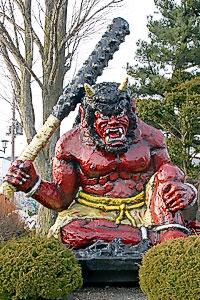
\includegraphics[width=1.4in]{Oni.jpg}

A picture of an Oni.
\end{center}
ONI provides a simple C API that simplifies the process of
implementing Overlog bindings for functions written in C.  It is
designed to be as simple as possible, and is currently incomplete.  If
you find that you need more functionality than is currently available,
email {\tt p2devel@yahoogroups.com}.

\subsection{A sample ONI stage}

Here is the C implementation of an ONI stage:
\begin{verbatim}
1  ONI_TUP_STAGE(hello_world) {
2    const char * str = str_Val(Val_Tup(tup,2));
3    const char * hello = "Hello ";
4    char * tmpstr = malloc(strlen(str)+strlen(hello)+1);
5    tmpstr[0] = 0;
6    strcat(tmpstr,hello);
7    strcat(tmpstr,str);
8    Tup_Push_str(tmpstr);
9    free(tmpstr);
10   return 0;
11 } END_ONI_STAGE
\end{verbatim}
The stage takes input tuples of the form \lstinline$(@loc, ``name'')$
and returns tuples of the form \lstinline$(@loc, ``Hello name'')$.
For now, all ONI stages produce exactly one output tuple for each
input tuple.  We plan to change this in future releases.

Lines 1 and 11 call C compiler macros, and define a function that will
be located and called by the ONI runtime.  The function defines two
variables of type {\tt tup\_t*}.  The first, {\tt tup}, is the input to
the stage.  The second, {\tt ret}, is the output tuple.

Line 2 unpacks the second value from the tuple, and performs a checked
cast to a C string.  ONI's interface to Overlog data structures
follows a simple naming convention.  Casting and accessor functions
are named {\tt foo\_bar()}, and produce something of type {\tt foo}
from something of type {\tt bar}.  For example, the call to {\tt
  str\_Val(...)} converts a P2 Value ({\tt val\_t*}) to a C-style
string ({\tt const char *}).  Similarly, {\tt Val\_Tup(tup,2)} returns
the third value in the tuple {\tt tup}.  ONI tuples are zero indexed.
P2 prepends a string containing the stage name to each input tuple.

Lines 3-7 are standard C string manipulation code.  Line 8 introduces
a new type of ONI function.  Functions that begin with {\tt Tup\_Push}
append a value to the end of a tuple.  Like the stage input tuple, all
tuples output by P2 stages must begin with a string containing the
name of the stage and a location specifier.  ONI automatically adds
these values to {\tt ret}.  If it did not, then we would need to
manually push them onto {\tt ret} before pushing the C string.

{\tt Tup\_Push\_str()} makes a copy of {\tt tmpstr}.  Line 9 frees the
now-unneeded copy of the C string.  Line 10 returns 0 to indicate
success.  Non-zero values are treated as internal errors in the P2
runtime.  For now, when a non-zero value is encountered, it is
reported to the user, and P2 immediately exits.  Errors that can be
handled in Overlog should be reported via the {\tt ret} tuple, and not
returned to ONI.

\subsection{ONI stage instantiation}
ONI stage instantiations look just like normal stage instantiations:
\begin{lstlisting}
stage("hello_world",hello_world_in,hello_world_out).
\end{lstlisting}
However, they are handled with a different set of runtime mechanisms.
Normal C++ stages are registered (at compile time) with {\tt
  stageRegistry.C}.  ONI stages are resolved at runtime by using C
dynamic linking.  Upon encountering a stage name that is unknown to
the {\tt StageRegistry}, P2 falls back on ONI's stage loader.  The
stage loader examines the stage name.  ONI stages are grouped into
modules according to a simple naming convention; all text before the
first ``{\tt\_}'' is treated as a module name.

Upon encountering a new module name, ONI attempts to open the
appropriate shared library and then searches the shared library's
symbol table for the correct stage implementation.  It would decide
that our hello\_world stage belongs in a module named ``hello''.
Under Linux, it would then attempt to {\tt dlopen()}
{\tt libonihello.so}\footnote{On Mac OS X, it still uses dlopen(), but
  looks for {\tt libonihello.dylib}.  Windows is not supported by ONI.},
and look for a function named ``{\tt \_Onihello\_worldFunc}''.  For
dynamic linking to succeed, {\tt libonihello.so} must be in a standard
shared library location ({\tt man dlopen} for more information), or in
a directory mentioned in {\tt LD\_LIBRARY\_PATH}.  Running

\begin{verbatim}
~/p2/build$ LD_LIBRARY_PATH=./oni ./tests/runStagedOverlog
    -o ../unitTests/olg/oniEcho.olg
\end{verbatim}
(all one line) will load and execute a sample ONI stage
under Linux and MacOS X.

{\em This is placeholder text:} The file {\tt oni/CMakeLists.txt}
builds a number of ONI stages.  For now, it is the best documentation
of ONI's compilation process.

\subsection{ONI {\em f\_functions}}

ONI does not support {\em f\_functions} yet.  ONI's C bindings into
P2's type system should transfer directly over to {\em f\_function}
implementations.  Adding ONI support for {\em f\_function}'s should be
matter of adding support for dynamic registration of new {\em f\_function}
definitions to P2.

\subsection{Manipulating Overlog types from C}

{\em This is placeholder text:} A number of other Overlog type
manipulation functions ({\tt int\_Val()}, {\tt Tup\_Push\_int()}, {\tt
  opaque\_Val()}, and {\tt Tup\_Push\_opaque()}) are available.  See
{\tt oni.h} for a current list.

Because of P2's heavy use of {\tt boost::shared\_ptr}, passing P2 {\tt
  Value}'s and {\tt Tuple}'s to and from C code is not entirely
straightforward.  The problem is that {\tt shared\_ptr} values cannot
be passed by value into C code.  This forces us to either obtain raw
pointers from P2's shared pointers (the current approach), or to pass
pointers to {\tt shared\_ptr}'s into the C code.  So far, we have
managed to hide P2's memory management from ONI bindings.  This
situation may change if we allow ONI to perform callbacks into P2.

A set of functions not mentioned above allow C code to allocate new P2
{\tt Value} objects.  It is unclear that these functions are needed, and
they may be removed in future releases. (Their names begin with ``{\tt
  alloc\_}'' and ``{\tt free\_}''.)  

Also, the Stasis ONI bindings (for which ONI was written) manipulate a
number of C structs.  The file {\tt oni/stasisTypes.C} provides some
examples of C struct packing and unpacking and other convenience
methods that may be instructive when developing Overlog bindings for
other C libraries that manipulate special-purpose data structures.

\subsection{The future of ONI}

ONI is in very early stages of development, and its API could change.
In the short term we plan to add support for more types of stages
(such as allowing ONI stages to produce variable numbers of tuples for
each input).

We are considering adding type-safe ONI stages.  The idea here is to
automatically generate the calls to {\tt str\_Val(), int\_Val(),
  etc.}, simplifying ONI bindings considerably, and (eventually)
exposing stage type information to the P2 runtime environment.

\section{PlanetLab Deployment}
\emph{This is placeholder text}

To use PlanetLab with a P2 application, please follow the following steps:

\begin{itemize}
\item Get a PlanetLab slice \texttt{<slice>}, find out your PlanetLab account
username \texttt{<username>}, and password \texttt{<password>}.
\item Compile P2 with the same libc setup as PlanetLab runs.  Currently
that is Fedora Core 4; later Fedora distributions run a later version of libc and
their executables will not run on PlanetLab.  Let \url{runOverLog} be that
executable. 
\item Figure out what OverLog program you'd like to run, and what
parametrizations you require (e.g., for landmark nodes and for other
nodes).  The example we will use is \url{doc/chord.olg}.
\item Figure out what parametrizations need to happen on each node.  To
automate this, produce a script \texttt{generator} in any language (we have
used python in this example) to figure out how to parametrize the
OverLog program. If you have no parametrizations, then just create an
empty script.  The command line interface to the script should be:
\begin{verbatim}
<generator> <sourceOverLogFilename> <random seed> <target hostname>
            <target port> <parametrizedOverLogFilename>
            [-Dkey=value]*
\end{verbatim}
In our example, \url{doc/chord.generator.py} is such a generator, whose task
is to take the input \url{doc/chord.olg} and set it to use a single node as
the landmark node, and set the node identifiers.
\item Use the \url{python/scripts/setupMonolithic.py} script to disseminate,
start, and stop your experiments on PlanetLab.  The script offers a
parallelism option (-j) whose argument determines how many nodes are
processed by the script at the same time. Leaving the option absent is
equivalent to "-j 1".  The script must have exactly one of 5 "actions":
-h gives the command line options. -a tells the script to pull in as
many nodes as it can to the slice given. -d removes all nodes from the
slice. -k kills the P2 process on all nodes given in the script.  -c
starts the P2 software on all nodes given in the script.
\begin{itemize}
\item Along with -c, the -i/-I option installs the necessary rpms on the
     given nodes (in the rpms/ directory)
\item If none of -z/-l options are given, all nodes in a slice will be
     included in an action.  -z excludes nodes.  -l only includes nodes
     explicitly.  Without -l, all nodes in the slice are included and
     then any mention in -z are excluded.
\item The script installs a short-term "ping port" to ensure all nodes
     have been installed appropriately.  By default, this is port 10001,
     but it can also set with the -t option.
\end{itemize}
Run the script as follows:

\begin{verbatim}
python python/scripts/setupMonolithic.py -n <slice> -o
<SourceOverlogFilename> -u <username> -w <password> -j <parallelism> -g
<generator script> [-Dkey=value]* -p portNumber -x <runOverLog>
[-z <excluded node>]* [-l <included node>]*  {-a|-d|-c|-k}  [-i] [-I]
\end{verbatim}

For example, to install and start P2-chord on all nodes in a slice do:

\begin{verbatim}
python python/scripts/setupMonolithic.py -n <slice> -o
doc/chord.olg -u <username> -w <password> -j 4 -g
doc/chord.generator.py -DLANDMARK=\"<landmarkNode>:10000\" -p 10000
-x <runOverLog> -c -I
\end{verbatim}

To run an updated version of chord.olg subsequently (without installing
new RPMs) do

\begin{verbatim}
python python/scripts/setupMonolithic.py -n <slice> -o
doc/chord.olg -u <username> -w <password> -j 4 -g
doc/chord.generator.py -DLANDMARK=\"<landmarkNode>:10000\" -p 10000
-x <runOverLog> -c
\end{verbatim}

To only start the landmark node do:

\begin{verbatim}
python python/scripts/setupMonolithic.py -n <slice> -o
doc/chord.olg -u <username> -w <password> -j 4 -g
doc/chord.generator.py -DLANDMARK=\"<landmarkNode>:10000\" -p 10000
-x <runOverLog> -c -l <landmarkNode>
\end{verbatim}

To only start everyone in the slice except the landmark node do:

\begin{verbatim}
python python/scripts/setupMonolithic.py -n <slice> -o
doc/chord.olg -u <username> -w <password> -j 4 -g
doc/chord.generator.py -DLANDMARK=\"<landmarkNode>:10000\" -p 10000
-x <runOverLog> -c -z <landmarkNode>
\end{verbatim}

To only start nodes n1, n2, and n3 do

\begin{verbatim}
python python/scripts/setupMonolithic.py -n <slice> -o
doc/chord.olg -u <username> -w <password> -j 4 -g
doc/chord.generator.py -DLANDMARK=\"<landmarkNode>:10000\" -p 10000
-x <runOverLog> -c -l n1 -l n2 -l n3
\end{verbatim}

To kill all P2 instances in the slice do

\begin{verbatim}
python python/scripts/setupMonolithic.py -n <slice> -o
doc/chord.olg -u <username> -w <password> -j 4 -g
doc/chord.generator.py -DLANDMARK=\"<landmarkNode>:10000\" -p 10000
-x <runOverLog> -k
\end{verbatim}

\item Output for the installation/shutdown of a P2 instance appears in the
start.log file on the target node.  Output of the P2 instance itself
(e.g., printouts, diagnostics, etc.) appear in the planetlab.log file on
the target node.
\end{itemize}

Note that the executable (\url{tests/runOverLog} in this case) would
best be a statically-linked executable (at least as far as the P2
libraries are concerned). To do that, configure your workspace as
follows before recompiling the entire distribution:
\begin{verbatim}
./configure LDFLAGS="-static" <other flags>
\end{verbatim}
Now all P2 libraries will be embedded statically in the executables;
other libraries might still be dynamically linked.  Make sure you
compile on an FC4 build server for PlanetLab experiments.





\section{Watches}
\label{sec:watches}

The \lstinline$watch$ and \lstinline$watchmod$ facts (of arity 1 and 2,
respectively) allow a programmer to place taps in
particular flows in the resulting dataflow graph.  For example 
\begin{lstlisting}
watch(eventName).
\end{lstlisting}
specifies that whenever eventName is produced, a line is appended to the
reporting stream of the runtime (e.g., on the standard output).  Watches
can have a modifier string, in which case the \lstinline$watchmod$ fact
is used.  For instance,
\begin{lstlisting}
watchmod(eventName, "id").
\end{lstlisting}
sets a watch on the \lstinline$eventName$ tuple type with modifiers
``i'' and ``d.''  An empty modifier string is equivalent to all
modifiers, so 
\begin{lstlisting}
watchmod(eventName, "").
\end{lstlisting}
is equivalent to the \lstinline$watch$ fact above.

Here are the different possible modifiers:
\begin{itemize}
\item InsertEvent, (i or INSERT\_EVENT), is issued right after a tuple is inserted into
  a table by the same name.
\item RefreshEvent, (r or REFRESH\_EVENT), is issued right after a tuple has been refreshed
  in a table by the same name.
\item DeleteEvent, (d or DELETE\_EVENT), is issued right after a tuple is deleted from a
  table by the same name.
\item RecvEvent, (c or RECV\_EVENT), is issued right after a tuple has been received from
  the network.
\item PeriodicEvent, p, is issued right after a periodic event has been issued.
\item AddAction, (a or ADD\_ACTION), is issued right before a tuple is inserted into the
  table by the same name.
\item DeleteAction, (z or DELETE\_ACTION), is issued right before a tuple is removed from
  the table by the same name.
\item SendAction, (s or SEND\_ACTION), is issued right before a tuple is transmitted.
\item BeforeJoin, b, is issued right before a tuple by that name is used
  to join with a table.
\item AfterJoin, j, is issued right after a join that created the tuple
  by that name.
\item HeadProjection, h, is issued right after a tuple by that name is
  produced as the head of a rule (within or without an aggregation rule).
\end{itemize}
Note that for the moment, the incremental planner only supports
modifiers that also have a long name.

An important note is that, though a tuple type may be received at a P2
node over the network, it may not be necessarily reported via
watches. This is the case when a tuple type is not \emph{expected} by
the node; that is, there is no rule taking that tuple type as its
input.  In that case, though the tuple may be received, it is
discarded.  To watch for such tuples, a workaround is to create a
reception rule that accepts the received tuple \lstinline$msg$ and produces a local
one \lstinline$gotMsg$.  Now watching for the sent tuple or the local
tuple will produce printouts.


\section{Language and System Limitations}
\begin{itemize}
\item At most one event per rule.
\item data import
\end{itemize}





\section{Known Bugs}

\begin{itemize}
\item Constants within predicates in the right hand side of a rule are
  ignored. For instance, rule 
\begin{lstlisting}
r1 action(@Me) :- predicate(@Me, 5).
\end{lstlisting}
is handled as indistinguishable from
\begin{lstlisting}
r1 action(@Me) :- predicate(@Me, _).
\end{lstlisting}
This is clearly a bug. For now, a workaround is to write
\begin{lstlisting}
r1 action(@Me) :- predicate(@Me, C), C == 5.
\end{lstlisting}
This bug does not apply to rule head predicates, so 
\begin{lstlisting}
r1 action(@Me, 5) :- predicate(@Me).
\end{lstlisting}
is handled correctly and the workaround is not required.
\end{itemize}



\section{P2DL: The P2 Dataflow Language}
\label{sec:p2dl}

\emph{Placeholder}

In this section, we describe the new P2 Dataflow Language (P2DL). The purpose
of this language is to serve as an intermediate compilation language for the
new P2 Overlog Compiler. In prior versions of the Overlog compiler, the dataflow
graph was created directly in the Planner. The result was complex code that only
few knew how to navigate. The complexity came from the need to directly create
and configure the C++ objects that make up the dataflow graph. The dataflow
language makes this a much more intuitive process by allowing for a syntactical 
representation of the dataflow graph.


\subsection{The Graph Description}

The {\bf graph} statement is how one creates an arbitrary graph out of
Elements. The statement has the following syntactical form.

\begin{verbatim}
graph <NAME> (<INPUTS>, <OUTPUTS>, <PROCESSING>, <FLOW_CODE>) {
     <GRAPH DESCRIPTION>
}
\end{verbatim}

A graph is declared using the {\bf graph} keyword followed by the {\em name}
of the graph. The graph name can be used to reference the graph in further
statements (more on this later). A graph statement requires four arguments.
\begin{enumerate}
\item INPUTS: The number of inputs to the graph.
\item OUTPUTS: The number of outputs to the graph.
\item PROCESSING: A string that defines the push/pull semantics of each input and output port.
\item FLOW\_CODE: A string defining the flow code semantics of each input and output port.
\end{enumerate}
The arguments to a graph are the same as those given to a basic P2 
Element~\footnote{In fact, in the new framework a dataflow object inherits 
from the Element class}. The graph statement corresponds to a dataflow 
object in the system, initialized according to the aforementioned arguments.

\subsubsection{Internal graph structure}

In this section we describe how to define the internal graph structure.
A graph specification describes a dataflow graph object that can be installed 
into the Plumber or used in another graph specification. The following is a 
simplified grammar of a graph specification.

\begin{verbatim}
graph <NAME> (<INPUTS>, <OUTPUTS>, <PROCESSING>, <FLOW_CODE>) {
     ( assignment; )*
     ( graph;}+
     ( strand; )+
}
.	# END OF PROGRAM
\end{verbatim}

The dataflow graph description is enclosed within brackets, and consists of a zero or more assignments, zero or more graph statements, and one or more dataflow strands.

\subsubsection{Assignments}
An assignment binds a variable to a P2 Element declaration and has the following 
syntax.

\begin{verbatim}
<variable> = <ELEMENT>( <arguments> );
\end{verbatim}

The variable can be any alpha or number character combination, and has a scope
within the graph statement. The above grammar binds the variable
to an Element object. The variable name can be used in strand statements to
specify the hookups that should be made to the binding Element object.

\subsubsection{Strand}
A strand defines how a set of elements and graphs are to be connected in the 
dataflow. A strand has the following simplified grammar. 

\begin{verbatim}
<element_expression> ( '->' <element_expression>)+;
\end{verbatim}

An element\_expression can be either the declaration of a new P2 Element, a 
variable, or the name of some previously defined graph.
The element\_expression can indicated the input/output ports that
are to be hooked up by the strand statement. If a port is not given then the hookup defaults to port zero. Ports a defined by enclosing the port identifier in square
brackets (e.g., [0] port zero, ["foo"] port "foo"). The position of the port identifier
indicates an input or an output. If the port identifier proceeds the element\_expression
then it is an input port. If it follows it is an output port identifier. The port identifier can
also indicate the addition of a new port~\footnote{Only to be used with Elements that
support dynamic port allocation.}. The [+] port identifier indicates the addition of a 
new port. If the port takes a string (e.g., the dynamic demux element) then 
the ["foo" +] port identifier would add the port string "foo" to the Element.


\subsubsection{Defining and Linking P2 Elements}
An element is defined by specifying the element type and any arguments required 
by the element constructor. Connecting two elements together is indicated by a link. 
The following sections define this process in more detail.

\subsubsection{Declaring P2 Elements}

An element is declared by specifying the Element type and any constructor arguments
defined by the actual P2 Element class. The argument types of a P2 element include
numeric (int or double), string, identifiers, and a C++ vector of P2 values. 
All of these types are supported in the P2DL. The support for P2 values and vector 
of P2 values will be described in Section~\ref{sec:p2values}. 

The first argument of a P2 element constructor is always the name the element. 
Under the general P2 architecture the element name can be
an arbitrary string. However, when using P2DL, in order to reference the element in an
edit the name of an element must follow the variable syntax by beginning with a lower
case alpha character.

\subsubsection{Hooking up P2 Elements using dataflow strands}

In the P2 architecture, elements are connected by linking together an output port
of one element to an input port of another element. The P2DL uses the array syntax
for specifying the port of an element. The following 'foobar'
graph description creates two Elements, TimedPushSource and Discard, and connects
the former output port 0 to the latter input port 0.

\begin{verbatim}
graph foobar (0, 0, "", "") {
         # No port specified defaults to port 0
         TimedPushSource("source", 1) -> Discard("discard");
}
.
\end{verbatim}

A dataflow strand is a series of P2 elements and links specifying how the element
ports should be connect. Each strand begins and ends with a single element\_expression
and is terminated with a semicolon. The input of the first element\_expression
and the output of the last element\_expression are not specified. Some elements 
require the configuration of multiple input/output ports, which can be supported by
declaring an element variable in the dataflow block and using that variable to reference
the Element object in multiple positions. 

\subsubsection{Declaring local variables using assignments}

Local variables provide a way
to reference an element\_expression in multiple positions, thereby permitting the 
configuration of any number of input/ouput ports. A local variable is defined
by assigning the Element declaration to a variable, as shown below.

\begin{verbatim}
graph bar(0, 0, "", "") {
         # Define local variable mux
         mux = Mux("mymux", 2);
         
         TimedPushSource("source1", 1) -> [0] mux[0] -> Discard("discard");
         TimedPushSource("source2", 1) -> [1] mux;
}
.
\end{verbatim}

\subsubsection{P2 values and vectors of P2 values}
\label{sec:p2values}

The values supported by P2DL include numeric (int, unsigned, and double), string,
identifier, and a vector of values. A numeric value in P2DL will create the appropriate
P2 value. An integer value is assumed to be an 'int' type unless a 'U' character is
appended to the value. An identifier is specified by appending a 'I' character to the
hexadecimal character string representing the identifier. A string value is indicated by enclosing
the string character with double quotes. A vector of values is indicated by enclosing
a list of values in brackets. The list of values is delimited with a comma. The following
provides some example vectors.
\begin{verbatim}
a = {0, 1, 2, 3};  # A list of integers
b = {0U, 1U, 2U, 3U}; # A list of unsigned integers
c = {1.0, 3.0}; # A list of double values
d = {"foo", "bar"}; # A list of string values
e = {2343254ef5e98I, 3e43545435454I}; # A list of identifers
f = Demux("mydemux", {"foo", "bar"});
g = Demux{"mysamedemux", d);
\end{verbatim} 

All examples above are expressed in assignment statements. The vector values
can be referenced by the binding variable in further statements. The assignment
to the variable 'f' binds that variable to a Demux object that is initialized with a vector of 
string values indicating the demux ports. The variable 'g' is also bound to a Demux
with the same configuration, but its vector values is provided by the variable 'd'.

\subsection{Edit Specification}
\label{sec:edits}

The edit construct is used for rewiring the elements of an installed dataflow graph. 
Permitting the ability to rewire a dataflow allows one to remove old elements 
and/or incorporate new elements into the dataflow graph. The following is a 
informal grammar to the edit specification.

\begin{verbatim}
edit <NAME> {
   (assignment;)*
   (graph;)*
   (strand;)+
}
\end{verbatim}

Every edit begins with the keyword {\bf edit}, followed by a DataflowName, which
must be the name of some dataflow that has already been installed in the 
Plumber~\footnote{Otherwise the Plumber will ignore the edit.}. The edit
block is enclosed in brackets and contains zero or more assignments and one or
more strands. The syntax for assignments remain the same but a dataflow strand
is now able to references elements of the dataflow being edited. A reference
to an existing element must be preceded by a single '.' in order to differentiate 
it from a local variable. The following example illustrates an edit on a dataflow
titled 'Main'.

\begin{verbatim}
edit main {
  main.marshal -> Bandwidth("bw") -> main.udp;
  main.cct -> main.unmarshal;  
}
.
\end{verbatim}

The first strand in the 'Main' edit rewires the output port $0$ of the existing element
named 'marshal' to the input port $0$ of a new 'Bandwidth' element. 
The output port $0$ of the new 'Bandwidth' element is connected to the existing element
named 'udp', which will result in a rewiring of the 'udp' element's input port $0$. The
second strand in the 'Main' edit rewires the output port $0$ of the existing 'cct' element
to the input port $0$ of the existing 'unmarshal' element.



 


\bibliographystyle{abbrv}
\bibliography{UserGuide}


\end{document}
